\subsection{\dechorate}

\begin{frame}{\dechorate: echo-aware dataset  \hfill\faTint}

    \alert{\iconAlert Everything so far was a simulation}

    \begin{mysotablock}{We need data}
        \begin{itemize}
            \item why?
            \item practice
            \item positioning acoustic
            \item expertise
        \end{itemize}

    \end{mysotablock}

    \begin{mycontriblock}{\dechorate: echo-aware dataset}
        \begin{itemize}
            \item different room configurations
            \\($to$ flipping wall panels)
            \item 6 array $\times$ 5 mics $\times$ 4 sources $\times$ 11 room conf. = 1320 annotated RIRs
            \item application to Room Geometry Estimation, Speech Enhancement and Acoustic Echo Retrieval
        \end{itemize}
    \hfill {\small \myThankTo{prof Gannot, ing. Tandeitnik}}
    \end{mycontriblock}

    % \begin{block}{\alert{Data} in audio signal processing}
    %     \begin{enumerate}
    %         \item typically RIRs
    %         \item necessary for validation/learning%for validating (and learning) models
    %         \item real data collection need expertise, equipment and time
    %         % \\\hspace{.3em} annotation and recording require expertise, equipment and \alert{time}
    %         \item dataset are for ad hoc setup
    %         % \\\hspace{.3em} they do not generalize to different use-cases and scenarios (array, recording scenario)
    %     \end{enumerate}

    %     \pause
    %     $\implies$ \alert{simulated data} are used instead $\implies$ \textcolor{myred}{validating/learning model with model}
    %     % quantity, versatility, annotation easiness and ``quality''
    % \end{block}

    % \pause
    % \begin{block}{\alert{Echo-aware real data} in audio signal processing}
    %     \vspace{-2mm}
    %     \begin{description}
    %         \item[For SE:] strong echoes\cmark, but not annotated\xmark, specific array\xmark
    %         \\{\small\cite{szoke2019building,bertin2019voicehome,remaggi2016acoustic}}
    %         \item[For RooGE:] good geom annotation\cmark, but a few acoustic scenarios\xmark
    %         \\{\small\cite{dokmanic2013acoustic,crocco2017uncalibrated,remaggi2019modeling}}
    %     \end{description}
    % \end{block}

    % \pause
    % \begin{center}
    %     \textcolor{myred}{A good echo-aware dataset should allow \textbf{SE}, \textbf{RooGE} and \textbf{AER}
    %     \\HOW?
    %     \\signal annotation \quad $\Longleftrightarrow$ \quad geometric annotation}
    % \end{center}

\end{frame}

\begin{frame}{\dechorate: echo-aware dataset \hfill\faTint}

    \begin{center}
        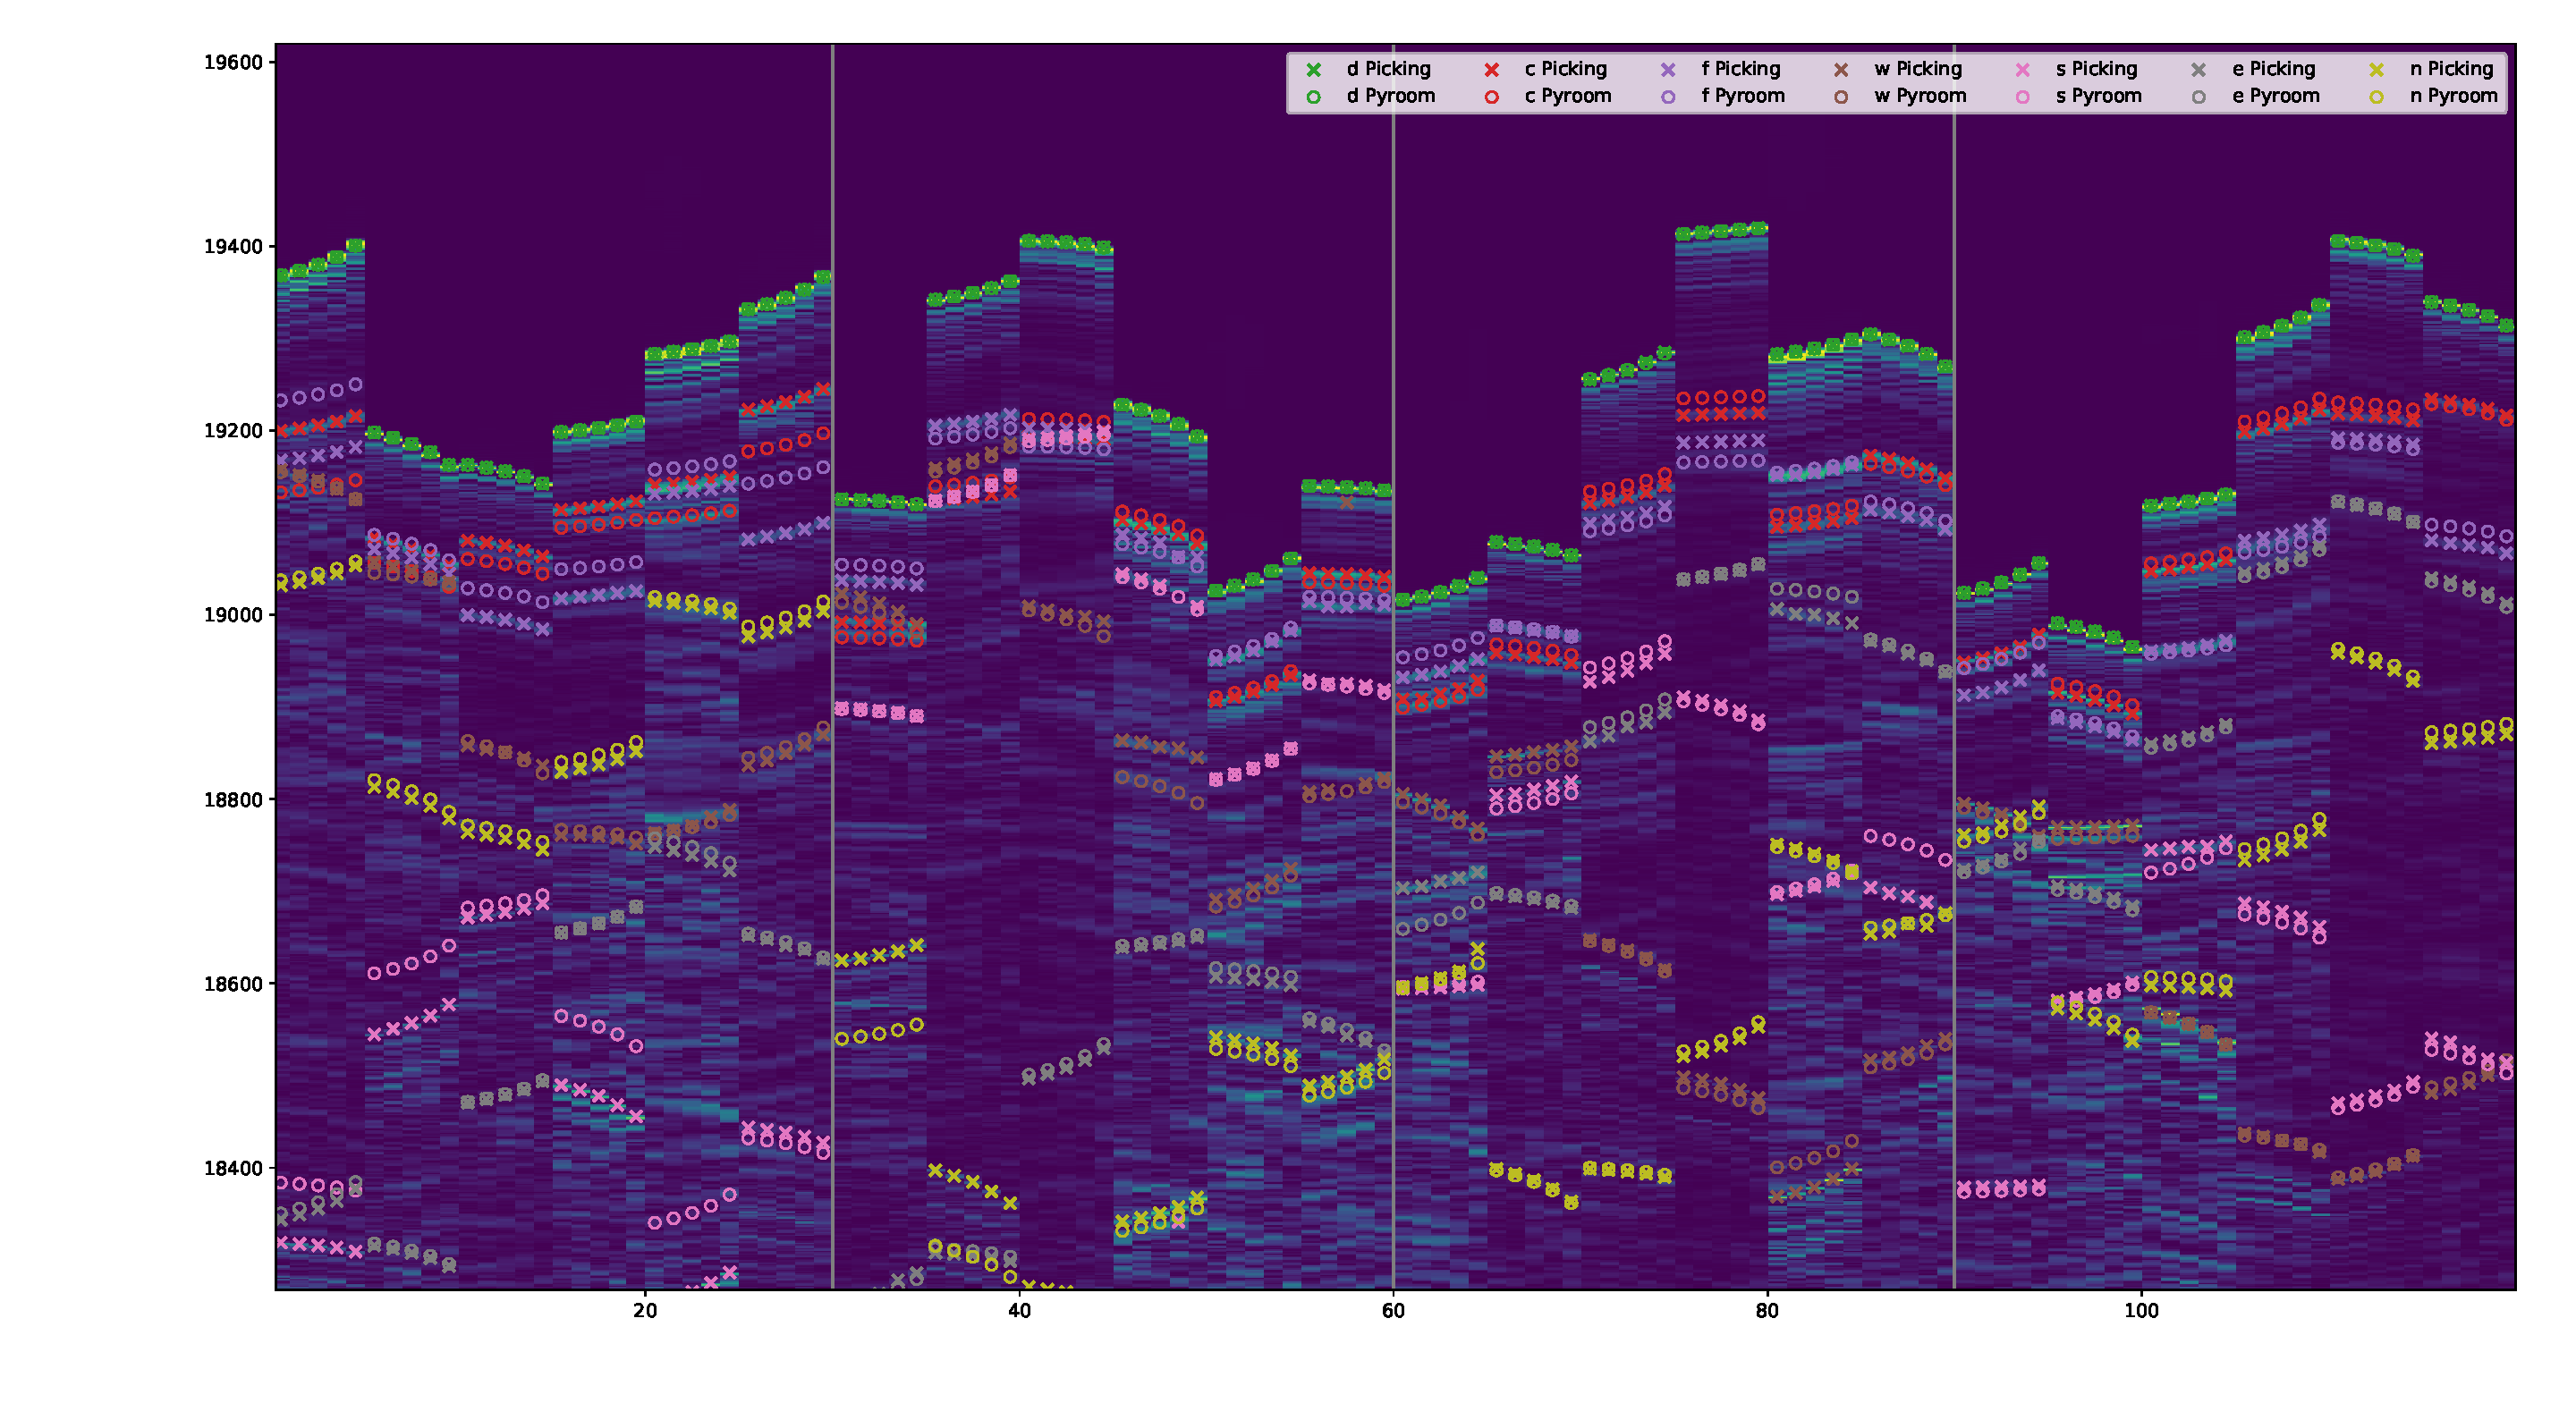
\includegraphics[trim={10em 0 0 0},clip,width=\linewidth]{figures/dechorate/rir_skyline_final_mod4paper.pdf}
    \end{center}

    \vspace*{-2mm}
    RIR Skyline showing
    \begin{itemize}
        \item absolute value of stacked RIRs as a figure
        \item[$\times$] manual echo annotation
        \item[$\circ$] \textit{matching} echo annotation for \texttt{ISM simulator}
    \end{itemize}
\end{frame}

\subsection{Speech Enhancement with \dechorate}

\begin{frame}[t]{Echo-aware Speech Enhancement with \dechorate}
    \begin{mydefblock}{Speech Enhancement (SE)}
        Improve the quality of a \alert{target} sound source w.r.t.:
        \begin{columns}[T,onlytextwidth]
            \column{0.3\textwidth}
                \centering
                \only<1>{interfering\\sources}\only<2->{\textcolor{gray}{interfering\\sources}}
                \\$\downarrow$
                \\source separation
            \column{0.05\textwidth}
            \centering
            +
            \column{0.3\textwidth}
                \centering
                \only<1>{noise}\only<2->{\alert{noise}}
                \\$\downarrow$
                \\denoising
            \column{0.05\textwidth}
                \centering
                +
            \column{0.3\textwidth}
                \centering
                \only<1>{reverberation}\only<2->{\alert{reverberation}}
                \\$\downarrow$
                \\dereverberation
                \\room equalization
        \end{columns}
    \end{mydefblock}

    \pause
    SE via \textbf{linear spatial filtering}
    \begin{columns}[onlytextwidth]
        \column{.3\textwidth}\centering
            $\bfh\bfs + \bfn = \bfx \in \bbC^{I}$
        \column{.05\textwidth}\centering
            $\longrightarrow$
        \column{.3\textwidth}\centering
        \begin{align*}
            \khermitian{\bfw} \in \bbC^{I} \\
        \end{align*}
        \column{.05\textwidth}\centering
        \begin{align*}
            \longrightarrow \\
        \end{align*}
        \column{.3\textwidth}\centering
        \begin{align*}
            \khermitian{\bfw} \bfx \approx \bfs \\
        \end{align*}
    \end{columns}

    \pause
    \begin{itemize}
        \small
        \item \textbf{target is distortionless} (vs. Multichannel Wiener Filtering)
        \item Partial \textit{steering vectors} from \textbf{geometry} \hspace{1em}\textcolor{gray}{\small(if anechoic $\implies$ DS based on AOA)}
        \item many variant, e.g. enhance or null multiple sources~\cite{gannot2017consolidated}
    \end{itemize}

    \pause
    \vfill
    \vspace*{.25em}
    \setbeamercolor{postit}{fg=black,bg=bluegreen!10}
    \begin{beamercolorbox}[sep=.5em]{postit}
        \centering
        \begin{equation*}
            \widehat{\bfw} = \underset{\bfw}{\arg\min} \;
            \bbE\kbrace{\set{ \kvvbar{\khermitian{\bfw} \bfx }_2^2}}
            \quad\text{s.t.}\quad\khermitian{\bfw}\bfh = 1
        \end{equation*}
        \textcolor{myred}{\small Reducing output energy + distortionless $\Leftrightarrow$ reduce any noise}
    \end{beamercolorbox}

\end{frame}

\begin{frame}[t]{Echo-aware Speech Enhancement}

    \begin{block}{Closed-form solution, but it requires:}
    \end{block}

    \vspace{-3mm}
    \begin{center}
        \begin{table*}
            \centering
            \small
            \begin{tabular}{llll}
                & Noise covariance matrix & Steering Vectors\\
                $\mathtt{DS}$                          &     -      & Direct Path (AOA)\\
                $\mathtt{MVDR}_\mathtt{DP}$            &   Noise    & Direct Path (AOA)\\
                $\mathtt{MVDR}_\mathtt{ReTF}$          &   Noise    & Relative Transfer Function\\
                \only<-2>{$\mathtt{MVDR}_\mathtt{Rake}$}%
                \only<3->{\alert{$\mathtt{MVDR}_\mathtt{Rake}}$}%
                            &   Noise    & Relative Early Echoes\\
                \visible<2->{%
                $\mathtt{MVDR}_\mathtt{DP+Late}$       &   Noise + Late Diffusion   & Direct Path (AOA)\\
                $\mathtt{MVDR}_\mathtt{ReTF+Late}$     &   Noise + Late Diffusion   & Relative Transfer Function\\
                \only<-2>{$\mathtt{MVDR}_\mathtt{Rake+Late}$}%
                \only<3->{\alert{$\mathtt{MVDR}_\mathtt{Rake+Late}$}}%
                            &   Noise + Late Diffusion   & Relative Early Echoes\\
                }
            \end{tabular}
        \end{table*}
    \end{center}

    \vspace{-3mm}
    \visible<4->{
    \begin{block}{Comparison on \dechorate data}
    \end{block}

    \begin{center}
        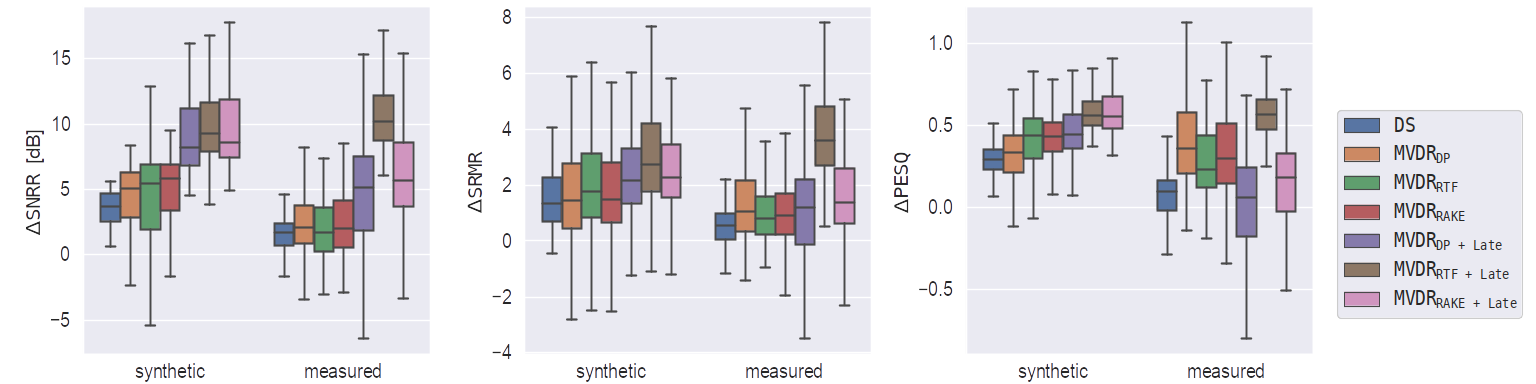
\includegraphics[width=\textwidth]{figures/dechorate/kowalkzy_results_boxplot_alpha.png}
    \end{center}
    }

    \vspace{-3mm}
    \visible<5->{
    \begin{itemize}
        \item<6-> \textit{In theory} echo-aware ws. echo-agnostic?
        \\$\to$ Better than Direct Path, but ReTF and Rake are comparable
        \item<7> Spatial filtering on Synthetic data vs. Measured data?
        \\$\to$ Rake suffer from mismatch, but better than DP
    \end{itemize}
    }
\end{frame}


% \subsection*{Interim conclusion (3/4)}

% \begin{frame}{Interim conclusion (3/4)}
%     \begin{block}{\dechorate dataset for echo-aware signal processing}
%         \begin{itemize}
%             \item designed for AER, SE and RooGE
%             \item Geometrical annotation $\longleftrightarrow$ image source annotation $\longleftrightarrow$ Signal Annotation
%             \item Measured Real RIRs and equivalent synt RIR
%             \item also speech, noise, babble noise and different room conf (+fornitures)
%             \item GUI, tools and code
%         \end{itemize}
%     \end{block}

%     \begin{block}{Application}
%         Echo Estimation
%         \begin{itemize}
%             \item Huge difference between real and simulated data
%         \end{itemize}
%         Room Geometry Reconstruction
%         \begin{itemize}
%             \item some annotation inconsistencies are noticed (but manually corrected)
%         \end{itemize}
%         Echo-aware Speech Enhancement
%         \begin{itemize}
%             \item a
%             \item b
%         \end{itemize}
%     \end{block}
% \end{frame}